\documentclass{beamer}
\usetheme{Madrid}

%------------------------------------------------------------------- PACKAGES -
\usepackage[brazil]{babel}
\usepackage[T1]{fontenc}
\usepackage[utf8]{inputenc}
\usepackage{colortbl}
\usepackage{multicol}

\usepackage{color}
\definecolor{cstrings}{rgb}{0.6,0,0}
\definecolor{ccomments}{rgb}{0.25,0.5,0.35}
\definecolor{ckeywords}{rgb}{0.25,0.35,0.75}

\usepackage{listings}
\lstset{language=C++,
basicstyle=\scriptsize\ttfamily,
keywordstyle=\color{ckeywords}\bfseries,
stringstyle=\color{cstrings},
commentstyle=\color{ccomments},
columns=fullflexible,}

%\includefile{c++}{pasta}{arquivo}
\newcommand\includefile[3]{\lstinputlisting[language=#1]{#2/#3}}


%---------------------------------------------------------------- DEFINITIONS -
%
%\def\dis{\displaystyle}
%\def\ol{\overline}
%\newcommand{\ang}[1]{\left\langle #1 \right\rangle}
%\newcommand{\transp}[2]{\input{#1#2}}
%
%\FontTitle{\large}{BW}
%FontTitle{\large}
%\hypersetup{pdfpagemode=FullScreen}


%---------------------------------------------------------------------- COVER -
\title[Treinos Livres]{Treinos Livres\\ Maratona de Programação}
\author[{\tiny André, Humberto, Paulo Cezar}]{André Augusto\\ Humberto Longo\\ Paulo Cezar Pereira Costa }
\institute[]{Instituto de Informática\\
           Universidade Federal de Goiás}
%\date[]{}

\newcommand{\bitem}{\item[\textbullet]}

\AtBeginSection[]
{
\begin{frame}<beamer>
\frametitle{}
\begin{center}
	\begin{minipage}{.9\textwidth}
	\begin{block}{}
		\centering
		\large
		\tt
		{\usebeamercolor[bg]{block title} \insertsection}
	\end{block}
	\end{minipage}
\end{center}
\end{frame}
}
\AtBeginSubsection[]
{
\begin{frame}<beamer>
\frametitle{}
\begin{center}
	\begin{minipage}{.9\textwidth}
	\begin{block}{}
		\centering
		\huge
		\tt
		{\usebeamercolor[bg]{block title} \insertsubsection}
	\end{block}
	\end{minipage}
\end{center}
\end{frame}
}


\begin{document}

\beamertemplatenavigationsymbolsempty
\maketitle


% ----------------------------------------------------------------------- AULA 2 ----------
%\section{Aula 2\ \ \ \ \ \ \ \ \ \ \ \ \ \ \ \ \ \ \ \ \ \ \ \ \ \ \ \ \ \ \ \ \ \ \ \ \ \ \ \ \ \ \ \ \  Noções de Complexidade, Problemas Ad Hoc e Estruturas de Dados}
%\subsection{Noções de Complexidade}
%%% formatação saída C++

%- - - - - - - - - - - - - - - - - - - - - - - - - - - - - - - - - NOCOES DE COMPLEXIDADE -
%- - - - - - - - - - - - - - - - - - - - - - - - - - - - - - - - - SLIDE -
\begin{frame}
\frametitle{Noções de Complexidade}

\begin{block}{Importância}
Além de dominar as diferentes técnicas  de solução de problemas, também é importante saber analisar a complexidade da sua solução.
\begin{itemize}
	\item[$\blacksquare$] Ninguém gosta de receber um \emph{Time Limit Exceeded}.
\end{itemize}
\end{block}

\begin{block}{}
\begin{table}
    \begin{tabular}{|l|l|l|l|l|l|l|}
        \hline
        Tamanho da entrada  & 10    & 20    & 50    & 100   & 1000   & 5000	\\ \hline
        algoritmo 1         & 0.00s & 0.01s & 0.05s & 0.47s & 23.92s & 47min	\\ \hline
        algoritmo 2         & 0.05s & 0.05s & 0.06s & 0.11s & 0.78s  & 14.22s	\\  \hline
    \end{tabular}
    \caption{Tempos de execução de dois algoritmos fictícios}
\end{table}
\end{block}
\end{frame}

%- - - - - - - - - - - - - - - - - - - - - - - - - - - - - - - - - SLIDE -
\begin{frame}
\frametitle{Noções de Complexidade}

\begin{block}{}
\begin{itemize}
	\item[] A solução de um problema deve ser eficiente.
	\item[] Dois possíveis jeitos de analisar a eficiência da sua solução:
	\begin{itemize}
		\bitem Implementar e executar medindo o tempo gasto (ou submeter e torcer pra não receber TLE).
		\item[\checkmark] Pensar no algoritmo e analisar o mesmo antes de começar a codificar.
	\end{itemize}
\end{itemize}
\end{block}

\begin{block}{}
Durante uma competição sabe-se os possíveis tamanhos da entrada. Supondo que um algoritmo foi pensado, algumas perguntas geralmente devem ser respondidas.
\begin{itemize}
	\bitem Vale a pena implementar essa solução? Ela vai resolver o maior caso em tempo?
	\bitem Sei mais de um algoritmo pra resolver um problema, qual devo implementar?
\end{itemize}
\end{block}
\end{frame}

%- - - - - - - - - - - - - - - - - - - - - - - - - - - - - - - - - SLIDE -
\begin{frame}
\frametitle{Noções de Complexidade}

\begin{block}{Certo, é importante. Mas como analisar a complexidade?}
\begin{itemize}
	\bitem Dois tipos de medida:
	\begin{itemize}
		\bitem Complexidade de Tempo -- nro. de operações executadas pelo algoritmo
		\bitem Complexidade de Espaço -- quantidade de memória que o algoritmo usa durante a execução 
	\end{itemize}
	\bitem Foco na análise da Complexidade de Tempo.
	\begin{itemize}
	\tiny
		\bitem Geralmente se o algoritmo tem uma boa complexidade de tempo, ele também tem uma boa complexidade de espaço.
		\bitem Costuma ser mais fácil estimar o espaço gasto.
	\end{itemize}
\end{itemize}
\end{block}

\begin{block}{Casos a serem levados em consideração}
\begin{itemize}
	\bitem Melhor caso
	\bitem Caso médio  
	\item[\checkmark]  Pior Caso
\end{itemize}
\end{block}

\end{frame}

%- - - - - - - - - - - - - - - - - - - - - - - - - - - - - - - - - SLIDE -
\begin{frame}
\frametitle{Noções de Complexidade}

\begin{block}{Análise assimptótica}
\begin{itemize}
	\bitem Considere o nro. de operações de cada um dos dois algoritmos fictícios que resolvem o mesmo problema uma função de $n$ (o ``tamanho'' da entrada)
	\begin{itemize}
		\bitem Algoritmo 1: $f_1(n) = 42n^2 + 13n$ operações
		\bitem Algoritmo 2: $f_2(n) = 1337n + 666$ operações
	\end{itemize}
	\bitem Dependendo do valor de $n$ o Algoritmo 1 pode requerer mais ou menos operações que o Algoritmo 2.
	\bitem Um caso de particular interesse é quando $n$ tem valor muito grande ($n \rightarrow \infty$), denominado comportamento assimptótico.
	\bitem Os termos inferiores e as constantes multiplicativas contribuem pouco na comparação e podem ser descartados.
\end{itemize}
\end{block}
\end{frame}

%- - - - - - - - - - - - - - - - - - - - - - - - - - - - - - - - - SLIDE -
\begin{frame}
\frametitle{Noções de Complexidade}

\begin{block}{Notação $O$}
\begin{itemize}
	\item[] Dada uma função $g(n)$, denotamos por $O(g(n))$ o conjunto das funções\\
		\begin{center}$\{f(n) : \exists$ constantes $c_1\ e\ n_0$ tais que $0 \leq f(n) \leq c_1g(n)$ para $n \geq n_0\}$\end{center}

	\item[] Isto é, para valores de $n$ suficientemente grandes, $f(n)$ é menor ou igual a $g(n)$.
	
	\begin{itemize}
		\bitem Algoritmo 1: $f_1(n) = 42n^2 + 13n \in O(n^2)$
		\bitem Algoritmo 2: $f_2(n) = 1337n + 666 \in O(n)$
	\end{itemize}
	
	\item[] Um polinômio de grau $d$ é de ordem $O(n^d)$. Como uma constante é considerada um polinômio de grau 0, dizemos que uma constante é $O(n^0)$, ou seja, $O(1)$.

	\begin{itemize}
	\tiny	
	\item[$\dagger$] $O(n) \times O(n) = O(n^2)$
	\item[$\dagger$] $O(n) + O(n) = O(n)$
	\item[$\dagger$] $O(n) + O(n^2) = O(n^2)$
	\end{itemize}
\end{itemize}
\end{block}
\end{frame}

%- - - - - - - - - - - - - - - - - - - - - - - - - - - - - - - - - SLIDE -
\begin{frame}
\frametitle{Noções de Complexidade}
\begin{block}{Exemplo: Selection Sort}

\begin{itemize}
	\item[] Para cada posição $i$ com $i$ variando de $0$ até $n-2$ \uncover<4->{$O(n)$}
	\begin{itemize}
		\item[] Encontre a posição $j$, ($i \leq j < n$) onde está o menor elemento. \uncover<3->{$O(n)$}
		\item[] Troque os valores das posições $i$ e $j$. \uncover<2->{$O(1)$}
	\end{itemize}
	\item[]<5-> $O(n) * (O(n) + O(1)) = O(n) * O(n) = O(n^2)$
\end{itemize}
\end{block}
\end{frame}

%- - - - - - - - - - - - - - - - - - - - - - - - - - - - - - - - - SLIDE -
\begin{frame}
\frametitle{Noções de Complexidade}

\begin{block}{Exemplo: Sequência de Fibonacci}
\begin{center}\textbf{1, 1, 2, 3, 5, 8, 13, 21, 34, ...}\end{center}
\begin{itemize}
	\item[] A sequência pode ser definida pela seguinte recorrência:
	\item[] $$F_n = \begin{cases}
					1&\text{se } n=1\\
					1&\text{se } n=2\\
					F_{n-1}+F_{n-2}&\text{se } n>2
				\end{cases}$$
\end{itemize}
\end{block}
\end{frame}

%- - - - - - - - - - - - - - - - - - - - - - - - - - - - - - - - - SLIDE -
\begin{frame}
\frametitle{Noções de Complexidade}

\begin{block}{Exemplo: Sequência de Fibonacci - Algoritmo 1}
\includefile{c++}{codes}{fib1.cpp}
\end{block}

\begin{block}{Exemplo: Sequência de Fibonacci - Algoritmo 2}
\includefile{c++}{codes}{fib2.cpp}
\end{block}
\end{frame}


%- - - - - - - - - - - - - - - - - - - - - - - - - - - - - - - - - SLIDE -
\begin{frame}
\frametitle{Noções de Complexidade}

\begin{block}{Exemplo: Sequência de Fibonacci - Algoritmo 1}
\includefile{c++}{codes}{fib1.cpp}
\end{block}

\begin{block}{Qual a complexidade?}
\begin{itemize}
	\bitem Inicialmente pode parecer que o número de operações dessa solução é constante, afinal no pior caso será feita uma verificação e uma soma.
	\bitem Mas, não podemos esquecer que essa é uma função recursiva, então esse número constante de operações será executado em cada chamada da função recursiva.
\end{itemize}
\end{block}
\end{frame}

%- - - - - - - - - - - - - - - - - - - - - - - - - - - - - - - - - SLIDE -
\begin{frame}
\frametitle{Noções de Complexidade}

\begin{block}{Exemplo: Sequência de Fibonacci - Algoritmo 1}
\includefile{c++}{codes}{fib1.cpp}
\end{block}
\begin{block}{Qual a complexidade?}
\begin{itemize}
	\bitem E como saber quantas chamadas serão feitas numa função?
	\begin{itemize}
		\bitem $O(x)$ possíveis valores para o parâmetro $y$ da função, 
		\bitem $b$ possíveis escolhas em cada chamada (fator de ramificação)
		\bitem $b^{O(x)}$ chamadas no pior caso
	\end{itemize}
	\bitem Para a solução em questão temos $O(2^n)$ possíveis chamadas com um custo $O(1)$
	\bitem Complexidade da solução: $O(2^n)$
\end{itemize}
\end{block}
\end{frame}

%- - - - - - - - - - - - - - - - - - - - - - - - - - - - - - - - - SLIDE -
\begin{frame}
\frametitle{Noções de Complexidade}

\begin{block}{Exemplo: Sequência de Fibonacci - Algoritmo 2}
\includefile{c++}{codes}{fib2.cpp}
\end{block}

\begin{block}{Qual a complexidade?}
$O(1)$ operações (\tiny \texttt{f[i] = f[i-1] + f[i-2];}\normalsize) sendo executadas $O(n)$ vezes.\\
Complexidade da solução: $O(n)$
\end{block}
\end{frame}

%- - - - - - - - - - - - - - - - - - - - - - - - - - - - - - - - - SLIDE -
\begin{frame}
\frametitle{Noções de Complexidade}

\begin{block}{Exemplo: Sequência de Fibonacci - Algoritmo 2}
\includefile{c++}{codes}{fib2.cpp}
\end{block}

\begin{block}{Qual a complexidade?}
E a complexidade de espaço?
\begin{itemize}
	\item[]<2-> $O(n)$
	\item[]<3-> Será que dá pra fazer melhor?
\end{itemize}
\end{block}
\end{frame}


%- - - - - - - - - - - - - - - - - - - - - - - - - - - - - - - - - SLIDE -
\begin{frame}
\frametitle{Noções de Complexidade}

\begin{block}{Exemplo: Sequência de Fibonacci - Uma terceira solução}
\includefile{c++}{codes}{fib3.cpp}
\end{block}

\begin{block}{Qual a complexidade?}
\begin{itemize}
	\item[] Complexidade de Tempo: $O(n)$
	\item[] Complexidade de Espaço: $O(1)$
\end{itemize}
\end{block}
\end{frame}

%- - - - - - - - - - - - - - - - - - - - - - - - - - - - - - - - - SLIDE -
\begin{frame}
\frametitle{Noções de Complexidade}

\begin{block}{Exemplo: Busca num vetor ordenado}
Problema: Dado um vetor de $n$ inteiros distintos, com os elementos em ordem crescente,
encontrar a posição onde está o valor $x$, ou informar que o mesmo não existe no vetor.\\
\end{block}
\pause
\begin{block}{Solução 1:}
\begin{itemize}
	\item[] Percorre o vetor comparando elemento por elemento até encontrar $x$
	\item[] Se olhou todos os elementos e não encontrou, $x$ não está presente.\\

	\bitem<3-> No pior caso todos os $n$ elementos são comparados
	\bitem<3-> $O(n)$
\end{itemize}
\end{block}

\end{frame}

%- - - - - - - - - - - - - - - - - - - - - - - - - - - - - - - - - SLIDE -
\begin{frame}
\frametitle{Noções de Complexidade}

\begin{block}{Exemplo: Busca num vetor ordenado}
Problema: Dado um vetor de $n$ inteiros distintos, com os elementos em ordem crescente,
encontrar a posição onde está o valor $x$, ou informar que o mesmo não existe no vetor.\\
\end{block}
\begin{block}{Solução 2:}
Mas o vetor está ordenado, será que isso não ajuda?
\uncover<2->
{
\begin{itemize}
\tiny
	\item[] Inicialmente procuramos nas posições \texttt{inicio = 0, fim = n-1}
	\item[] enquanto inicio <= fim
	\begin{itemize}
\tiny
		\item[] \texttt{meio = (inicio+fim)/2}
		\item[] se \texttt{array[ meio ] < x}, \texttt{inicio = meio + 1;}
		\item[] se \texttt{array[ meio ] > x,} \texttt{fim = meio - 1;}
		\item[] se \texttt{array[ meio ] == x}, Encontrou $x$ na posição 'meio' 
	\end{itemize}
	\item[] $x$ não está presente no vetor
\normalsize
	\bitem<3-> Como a faixa onde estamos buscando o valor vai ser sempre dividida ao meio, no máximo $O(log_2\ n)$ faixas são verificadas.
	\bitem<3-> Complexidade da solução: $O(log\ n)$
\end{itemize}
}
\end{block}

\end{frame}





%\subsection{Problemas Ad Hoc}
%%- - - - - - - - - - - - - - - - - - - - - - - - - - - - - - - - - PROBLEMAS AD HOC -
%- - - - - - - - - - - - - - - - - - - - - - - - - - - - - - - - - SLIDE -
\begin{frame}
\frametitle{Problemas Ad Hoc}
\begin{block}{O que são?}
\begin{itemize}
	\bitem Problemas ``Ad Hoc'' são aqueles cuja solução não utiliza nenhum algoritmo bem conhecido.
	\bitem Cada problema ``Ad Hoc'' é diferente e tem uma solução específica.
	\bitem Geralmente esses problemas são os mais divertidos (e as vezes os mais frustrantes) já que cada um apresenta um novo desafio.
	\bitem A solução pode envolver uma estrutura de dados singular ou um conjunto incomum de loops e/ou condicionais.
	\bitem Não exclui o uso de outras técnicas.
\end{itemize}
\end{block}
\end{frame}
%- - - - - - - - - - - - - - - - - - - - - - - - - - - - - - - - - SLIDE -
\begin{frame}
\frametitle{Problemas Ad Hoc}
\begin{center}
	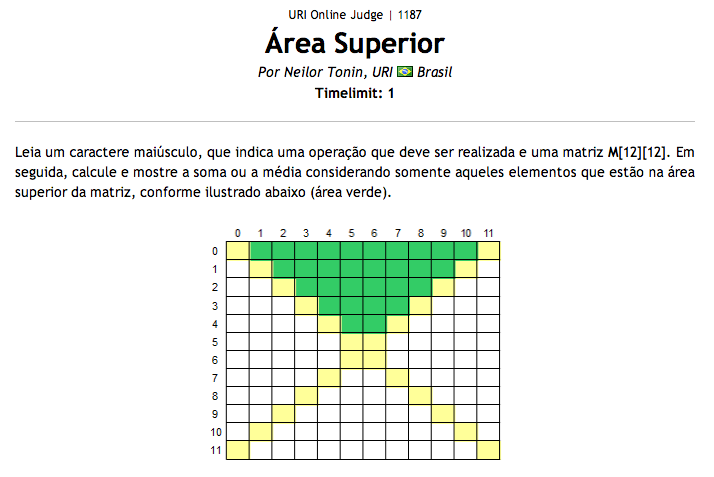
\includegraphics[width=.85\textwidth]{figuras/URI-1187.png}
\end{center}
\end{frame}	

%\subsection{Estruturas de Dados Básicas}
%%- - - - - - - - - - - - - - - - - - - - - - - - - - - - - - - - - ESTRUTURAS DE DADOS -
%- - - - - - - - - - - - - - - - - - - - - - - - - - - - - - - - - SLIDE -

% array static / vector ..
% problema / motivação
%    recuperar um valor de acordo com diferentes politicas
% 	 stack
% 	 queue
% 	 PQ
% C++ String
% BST -- set, map
% STL - sort, algorithm...


\begin{frame}
\frametitle{Estruturas de Dados Básicas}
\begin{block}{Objetivo}
Apresentar algumas estruturas de dados básicas e comumente usadas em competições.
\begin{itemize}
	\bitem Foco na aplicação das mesmas, utilizando a \emph{Standard Library} do C++.
\end{itemize}
\end{block}
\end{frame}

%- - - - - - - - - - - - - - - - - - - - - - - - - - - - - - - - - SLIDE -
\begin{frame}
\frametitle{Estruturas de Dados Básicas}
\begin{block}{Vetores}
\begin{itemize}
	\bitem Vetor estático -- \texttt{int array[256];}
	\bitem Vetor dinâmico 
	\begin{itemize}
		\bitem C++ \emph{Standard Library} \textbf{vector}, Java \textbf{Vector}
	\end{itemize}
\end{itemize}
\end{block}

\begin{block}{STL vector}
\begin{itemize}
	\item[] \texttt{\#include<vector>}
	\begin{itemize}
		\item[] \texttt{vector<int> a;    a.push\_back(x); }
		\item[] \texttt{vector<int> a(15);  a[10] = 42;}
		\item[] \texttt{vector<int> a(15, -1);}
		\item[] \texttt{vector<char> b; vector<double> c;}
		\item[] \texttt{vector<int> a; a.resize(1337); }
	\end{itemize}
\end{itemize}
\end{block}
\end{frame}

%- - - - - - - - - - - - - - - - - - - - - - - - - - - - - - - - - SLIDE -
\defverbatim[colored]\lstI{
\begin{lstlisting}[language=C++]
void semestre() {
	while(true) { /* nunca para */
		tarefa x = PegaNovaTarefa(tarefas);
		processa(x);
		/* novas tarefas podem surgir */
	}
}
\end{lstlisting}
}


\begin{frame}
\frametitle{Estruturas de Dados Básicas}
\begin{block}{Semestre típico}
\lstI
\end{block}

\begin{block}{}
	\begin{itemize}
		\bitem PegaNovaTarefa() decide a ordem em que as tarefas serão selecionadas.
	\end{itemize}
\end{block}

\end{frame}

%- - - - - - - - - - - - - - - - - - - - - - - - - - - - - - - - - SLIDE -
\begin{frame}
\frametitle{Estruturas de Dados Básicas}
\begin{block}{PegaNovaTarefa()}
\begin{itemize}
	\bitem Possíveis comportamentos de PegaNovaTarefa():
	\begin{itemize}
		\bitem Retorna a tarefa mais nova
		\bitem Retorna a tarefa mais velha
		\bitem Retorna a tarefa mais urgente
		\bitem Retorna a tarefa mais fácil
	\end{itemize}
	\bitem Queremos que PegaNovaTarefa() execute no menor tempo possível:
	\begin{itemize}
		\bitem ... organizando as tarefas de uma forma inteligente
	\end{itemize}
\end{itemize}
\end{block}
\end{frame}

%- - - - - - - - - - - - - - - - - - - - - - - - - - - - - - - - - SLIDE -
\begin{frame}
\frametitle{Estruturas de Dados Básicas}
\begin{block}{PegaNovaTarefa()}
\begin{itemize}
	\bitem Possíveis comportamentos de PegaNovaTarefa():
	\begin{itemize}
		\bitem Retorna a tarefa mais nova (pilha)
		\bitem Retorna a tarefa mais velha
		\bitem Retorna a tarefa mais urgente
		\bitem Retorna a tarefa mais fácil
	\end{itemize}
	\bitem Queremos que PegaNovaTarefa() execute no menor tempo possível:
	\begin{itemize}
		\bitem ... organizando as tarefas de uma forma inteligente
	\end{itemize}
\end{itemize}
\end{block}
\end{frame}

%- - - - - - - - - - - - - - - - - - - - - - - - - - - - - - - - - SLIDE -
\begin{frame}
\frametitle{Estruturas de Dados Básicas}
\begin{block}{Pilha}
\begin{itemize}
	\bitem Ultimo que entra é o primeiro que sai (LIFO)
	\bitem Suporta três operações de tempo constante:
	\begin{itemize}
		\bitem Push(x): Insere x na pilha
		\bitem Pop(): Remove o item mais novo
		\bitem Top(): Retorna o item mais novo
	\end{itemize}
	\bitem Implementação pronta na STL (stack)
\end{itemize}
\end{block}
\end{frame}

%- - - - - - - - - - - - - - - - - - - - - - - - - - - - - - - - - SLIDE -
\begin{frame}
\frametitle{Estruturas de Dados Básicas}
\begin{block}{STL - Stack}
\begin{itemize}
	\bitem empty() Testa se a pilha está vazia
	\begin{itemize}
		\bitem Complexidade - $O(1)$
	\end{itemize}
	\bitem size() Retorna o tamanho da pilha
	\begin{itemize}
		\bitem Complexidade - $O(1)$
	\end{itemize}
	\bitem top() Retorna o topo da pilha
	\begin{itemize}
		\bitem Complexidade - $O(1)$
	\end{itemize}
	\bitem push(elemento) Insere um elemento na pilha
	\begin{itemize}
		\bitem Complexidade - $O(1)$
	\end{itemize}
	\bitem pop() Retira um elemento da pilha
	\begin{itemize}
		\bitem Complexidade - $O(1)$
	\end{itemize}
\end{itemize}
\end{block}
\end{frame}

%- - - - - - - - - - - - - - - - - - - - - - - - - - - - - - - - - SLIDE -
\begin{frame}
\frametitle{Estruturas de Dados Básicas}
\begin{block}{PegaNovaTarefa()}
\begin{itemize}
	\bitem Possíveis comportamentos de PegaNovaTarefa():
	\begin{itemize}
		\bitem Retorna a tarefa mais nova (pilha)
		\bitem Retorna a tarefa mais velha
		\bitem Retorna a tarefa mais urgente
		\bitem Retorna a tarefa mais fácil
	\end{itemize}
	\bitem Queremos que PegaNovaTarefa() execute no menor tempo possível:
	\begin{itemize}
		\bitem ... organizando as tarefas de uma forma inteligente
	\end{itemize}
\end{itemize}
\end{block}
\end{frame}

%- - - - - - - - - - - - - - - - - - - - - - - - - - - - - - - - - SLIDE -
\begin{frame}
\frametitle{Estruturas de Dados Básicas}
\begin{block}{PegaNovaTarefa()}
\begin{itemize}
	\bitem Possíveis comportamentos de PegaNovaTarefa():
	\begin{itemize}
		\bitem Retorna a tarefa mais nova (pilha)
		\bitem Retorna a tarefa mais velha (fila)
		\bitem Retorna a tarefa mais urgente
		\bitem Retorna a tarefa mais fácil
	\end{itemize}
	\bitem Queremos que PegaNovaTarefa() execute no menor tempo possível:
	\begin{itemize}
		\bitem ... organizando as tarefas de uma forma inteligente
	\end{itemize}
\end{itemize}
\end{block}
\end{frame}

%- - - - - - - - - - - - - - - - - - - - - - - - - - - - - - - - - SLIDE -
\begin{frame}
\frametitle{Estruturas de Dados Básicas}
\begin{block}{Fila}
\begin{itemize}
	\bitem Primeiro que entra é o primeiro que sai (FIFO)
	\bitem Suporta três operações de tempo constante:
	\begin{itemize}
		\bitem Push(x): Insere x na fila
		\bitem Pop(): Remove o item mais velho
		\bitem Front(): Retorna o item mais velho
	\end{itemize}
	\bitem Implementação pronta na STL (queue)
\end{itemize}
\end{block}
\end{frame}

%- - - - - - - - - - - - - - - - - - - - - - - - - - - - - - - - - SLIDE -
\begin{frame}
\frametitle{Estruturas de Dados Básicas}
\begin{block}{STL - Queue}
\begin{itemize}
	\bitem empty() Testa se a fila está vazia
	\begin{itemize}
		\bitem Complexidade - $O(1)$
	\end{itemize}
	\bitem size() Retorna o tamanho da fila
	\begin{itemize}
		\bitem Complexidade - $O(1)$
	\end{itemize}
	\bitem front() Retorna quem está na frente da fila
	\begin{itemize}
		\bitem Complexidade - $O(1)$
	\end{itemize}
	\bitem back() Retorna quem está no fim da fila
	\begin{itemize}
		\bitem Complexidade - $O(1)$
	\end{itemize}
	\bitem push(elemento) Insere um elemento na fila
	\begin{itemize}
		\bitem Complexidade - $O(1)$
	\end{itemize}
	\bitem pop() Retira um elemento da fila
	\begin{itemize}
		\bitem Complexidade - $O(1)$
	\end{itemize}
\end{itemize}
\end{block}
\end{frame}

%- - - - - - - - - - - - - - - - - - - - - - - - - - - - - - - - - SLIDE -
\begin{frame}
\frametitle{Estruturas de Dados Básicas}
\begin{block}{PegaNovaTarefa()}
\begin{itemize}
	\bitem Possíveis comportamentos de PegaNovaTarefa():
	\begin{itemize}
		\bitem Retorna a tarefa mais nova (pilha)
		\bitem Retorna a tarefa mais velha (fila)
		\bitem Retorna a tarefa mais urgente
		\bitem Retorna a tarefa mais fácil
	\end{itemize}
	\bitem Queremos que PegaNovaTarefa() execute no menor tempo possível:
	\begin{itemize}
		\bitem ... organizando as tarefas de uma forma inteligente
	\end{itemize}
\end{itemize}
\end{block}
\end{frame}

%- - - - - - - - - - - - - - - - - - - - - - - - - - - - - - - - - SLIDE -
\begin{frame}
\frametitle{Estruturas de Dados Básicas}
\begin{block}{PegaNovaTarefa()}
\begin{itemize}
	\bitem Possíveis comportamentos de PegaNovaTarefa():
	\begin{itemize}
		\bitem Retorna a tarefa mais nova (pilha)
		\bitem Retorna a tarefa mais velha (fila)
		\bitem Retorna a tarefa mais urgente (fila de prioridades)
		\bitem Retorna a tarefa mais fácil
	\end{itemize}
	\bitem Queremos que PegaNovaTarefa() execute no menor tempo possível:
	\begin{itemize}
		\bitem ... organizando as tarefas de uma forma inteligente
	\end{itemize}
\end{itemize}
\end{block}
\end{frame}

%- - - - - - - - - - - - - - - - - - - - - - - - - - - - - - - - - SLIDE -
\begin{frame}
\frametitle{Estruturas de Dados Básicas}
\begin{block}{PegaNovaTarefa()}
\begin{itemize}
	\bitem Possíveis comportamentos de PegaNovaTarefa():
	\begin{itemize}
		\bitem Retorna a tarefa mais nova (pilha)
		\bitem Retorna a tarefa mais velha (fila)
		\bitem Retorna a tarefa mais urgente (fila de prioridades)
		\bitem Retorna a tarefa mais fácil (fila de prioridades)
	\end{itemize}
	\bitem Queremos que PegaNovaTarefa() execute no menor tempo possível:
	\begin{itemize}
		\bitem ... organizando as tarefas de uma forma inteligente
	\end{itemize}
\end{itemize}
\end{block}
\end{frame}

%- - - - - - - - - - - - - - - - - - - - - - - - - - - - - - - - - SLIDE -
\begin{frame}
\frametitle{Estruturas de Dados Básicas}
\begin{block}{Fila de prioridades}
\begin{itemize}
	\bitem Cada elemento em uma fila de prioridades tem um valor que corresponde a sua prioridade
	\bitem Suporta três operações
	\begin{itemize}
		\bitem Push(x, p): Insere x com prioridade p na fila de prioridades
		\bitem Pop(): Remove o elemento com a maior prioridade
		\bitem Top(): Retorna o elemento com a maior prioridade
	\end{itemize}
	\bitem Todas as operações podem ser feitas de forma rápida se implementadas usando uma Heap
	\bitem Implementação com Heap pronta na STL (priority\_queue)
\end{itemize}
\end{block}
\end{frame}

%- - - - - - - - - - - - - - - - - - - - - - - - - - - - - - - - - SLIDE -
\begin{frame}
\frametitle{Estruturas de Dados Básicas}
\begin{block}{STL - Priority Queue}
\begin{itemize}
	\bitem empty() Testa se a fila está vazia
	\begin{itemize}
		\bitem Complexidade - $O(1)$
	\end{itemize}
	\bitem size() Retorna o tamanho da fila
	\begin{itemize}
		\bitem Complexidade - $O(1)$
	\end{itemize}
	\bitem top() Retorna a frente da fila
	\begin{itemize}
		\bitem Complexidade - $O(1)$
	\end{itemize}
	\bitem push(element) Insere um elemento na fila
	\begin{itemize}
		\bitem Complexidade - $O(log\ n)$
	\end{itemize}
	\bitem pop() Retira um elemento da fila
	\begin{itemize}
		\bitem Complexidade - $O(log\ n)$
	\end{itemize}
\end{itemize}
\end{block}
\end{frame}

%- - - - - - - - - - - - - - - - - - - - - - - - - - - - - - - - - SLIDE -
\begin{frame}
\frametitle{Estruturas de Dados Básicas}
\begin{block}{Binary Search Tree}
	\begin{itemize}
		\bitem É uma árvore binária com a seguinte propriedade: para cada nó $v$,
		\begin{itemize}
			\bitem o valor de $v \geq$ valores na subárvore esquerda de $v$
			\bitem  o valor de $v \leq$ valores na subárvore direita de $v$
		\end{itemize}
	\end{itemize}

	\begin{center}
		\begin{figure}
			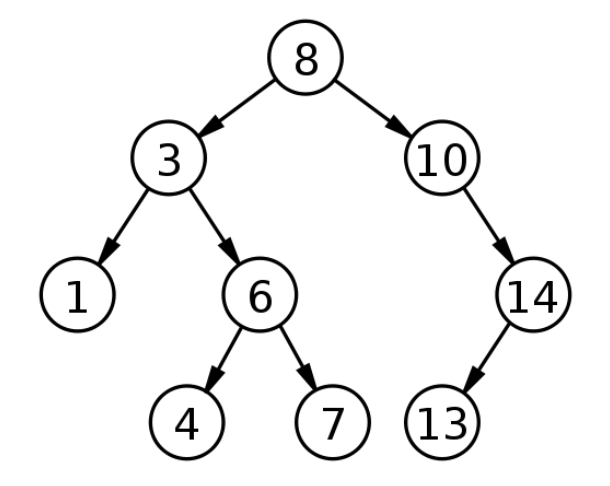
\includegraphics[width=.42\textwidth]{figuras/BST.png}
			\caption{Wikipédia}
		\end{figure}
	\end{center}
\end{block}
\end{frame}

%- - - - - - - - - - - - - - - - - - - - - - - - - - - - - - - - - SLIDE -
\begin{frame}
\frametitle{Estruturas de Dados Básicas}
\begin{block}{Binary Search Tree - O que elas podem fazer}
	\begin{itemize}
		\bitem Suporta três operações
		\begin{itemize}
			\bitem Insere(x): insere um nó com valor x
			\bitem Deleta(x): delete um nó com valor x, se o mesmo existir
			\bitem Encontra(x): retorna o nó com valor x, se o mesmo existir
		\end{itemize}
		\bitem Várias extensões são possíveis
		\begin{itemize}
			\bitem Conte(x): conta o número de nós com valor $\leq$ x
			\bitem PegaProximo(x): retorna o menor nó com valor $\geq$ x
		\end{itemize}
	\end{itemize}
\end{block}
\end{frame}

%- - - - - - - - - - - - - - - - - - - - - - - - - - - - - - - - - SLIDE -
\begin{frame}
\frametitle{Estruturas de Dados Básicas}
\begin{block}{Binary Search Tree - Competições de Programação}
	\begin{itemize}
		\bitem Uma implementação simples não garante a eficiência
		\begin{itemize}
			\bitem No pior caso, a altura da árvore se torna $n$ (o que faz a BST inútil)
			\bitem Garantir complexidade de tempo $O(log\ n)$ por operação requer um balanceamento da árvore (difícil de implementar)
			\bitem Vamos pular os detalhes de implementação
		\end{itemize}
		\bitem Use as implementações prontas da STL!
		\begin{itemize}
			\bitem set, map \textbf{(C++)}
		\end{itemize}
	\end{itemize}
\end{block}
\end{frame}

%- - - - - - - - - - - - - - - - - - - - - - - - - - - - - - - - - SLIDE -
\begin{frame}
\frametitle{Estruturas de Dados Básicas}
\begin{block}{STL - Set}
\begin{itemize}
	\bitem empty() Testa se o set está vazio
	\begin{itemize}
		\bitem Complexidade - $O(1)$
	\end{itemize}
	\bitem size() Retorna o tamanho do set
	\begin{itemize}
		\bitem Complexidade - $O(1)$
	\end{itemize}
	\bitem insert(elemento) Insere um elemento no set
	\begin{itemize}
		\bitem Complexidade - $O(log\ n)$
	\end{itemize}
	\bitem erase(element) Deleta um elemento do set
	\begin{itemize}
		\bitem Complexidade - $O(log\ n)$
	\end{itemize}
	\bitem clear() Limpa o set
	\begin{itemize}
		\bitem Complexidade - $O(n)$
	\end{itemize}
\end{itemize}
\end{block}
\end{frame}

%- - - - - - - - - - - - - - - - - - - - - - - - - - - - - - - - - SLIDE -
\begin{frame}
\frametitle{Estruturas de Dados Básicas}
\begin{block}{STL - Map}
\begin{itemize}
	\bitem empty() Testa se o map está vazio
	\begin{itemize}
		\bitem Complexidade - $O(1)$
	\end{itemize}
	\bitem size() Retorna o tamanho do map
	\begin{itemize}
		\bitem Complexidade - $O(1)$
	\end{itemize}
	\bitem insert(elemento) Insere um elemento no map
	\begin{itemize}
		\bitem Complexidade - $O(log\ n)$
	\end{itemize}
	\bitem erase(element) Deleta um elemento do map
	\begin{itemize}
		\bitem Complexidade - $O(log\ n)$
	\end{itemize}
	\bitem clear() Limpa o set
	\begin{itemize}
		\bitem Complexidade - $O(n)$
	\end{itemize}
\end{itemize}
\end{block}
\end{frame}

%- - - - - - - - - - - - - - - - - - - - - - - - - - - - - - - - - SLIDE -
\begin{frame}
\frametitle{STL - Funções úteis}
\begin{block}{cctype}
\begin{itemize}
	\bitem Funções determinantes de propriedades dos caracteres: isalnum, isalpha, isblank, iscntrl, isdigit, isgraph, islower, isprint, ispunct, isspace, isupper, isxdigit
	\bitem Funções de conversão: tolower, toupper
\end{itemize}
\end{block}
\end{frame}

%- - - - - - - - - - - - - - - - - - - - - - - - - - - - - - - - - SLIDE -
\begin{frame}
\frametitle{STL - Funções úteis}
\begin{block}{algorithm}
\begin{itemize}
	\bitem swap, unique, reverse, sort, lower\_bound, upper\_bound, binary\_search, set\_intersection, min, max, min\_element, max\_element, next\_permutation, prev\_permutation ...
\end{itemize}
\end{block}
\end{frame}

%- - - - - - - - - - - - - - - - - - - - - - - - - - - - - - - - - SLIDE -
\begin{frame}
\frametitle{STL - Funções úteis}
\begin{block}{cmath}
\begin{itemize}
	\bitem cos, sin, tan, acos, asin, atan, atan2, log, log10, sqrt, ceil, floor...
\end{itemize}
\end{block}
\end{frame}

%- - - - - - - - - - - - - - - - - - - - - - - - - - - - - - - - - SLIDE -
\begin{frame}
\frametitle{Leituras Recomendadas}

\begin{block}{}
\begin{itemize}
\tiny
	\bitem \url{http://community.topcoder.com/tc?module=Static&d1=tutorials&d2=complexity1}
	\bitem \url{http://community.topcoder.com/tc?module=Static&d1=tutorials&d2=complexity2}
	\bitem \url{http://www.inf.ufg.br/~cc080153/tap/material/stl_part1.pdf}
	\bitem \url{http://www.inf.ufg.br/~cc080153/tap/material/stl_part2.pdf}
	\bitem \url{http://www.inf.ufg.br/~cc080153/tap/material/stl_part3.pdf}	
	\bitem \url{http://community.topcoder.com/tc?module=Static&d1=tutorials&d2=dataStructures}
%	\bitem \url{http://community.topcoder.com/tc?module=Static&d1=tutorials&d2=bitManipulation}
	\bitem \url{http://community.topcoder.com/tc?module=Static&d1=tutorials&d2=standardTemplateLibrary}
	\bitem \url{http://community.topcoder.com/tc?module=Static&d1=tutorials&d2=standardTemplateLibrary2}
\end{itemize}
\end{block}

\end{frame}

%%- - - - - - - - - - - - - - - - - - - - - - - - - - - - - - - - - ESTRUTURAS DE DADOS -
%%- - - - - - - - - - - - - - - - - - - - - - - - - - - - - - - - - SLIDE -
%
%% array static / vector ..
%% problema / motivação
%%    recuperar um valor de acordo com diferentes politicas
%% 	 stack
%% 	 queue
%% 	 PQ
%% C++ String
%% BST -- set, map
%% STL - sort, algorithm...
%
%
%\begin{frame}
%\frametitle{Estruturas de Dados Básicas}
%\begin{block}{Objetivo}
%Apresentar algumas estruturas de dados básicas e comumente usadas em competições.
%\begin{itemize}
%	\bitem Foco na aplicação das mesmas, utilizando a \emph{Standard Library} do C++.
%\end{itemize}
%\end{block}
%\end{frame}
%
%%- - - - - - - - - - - - - - - - - - - - - - - - - - - - - - - - - SLIDE -
%\begin{frame}
%\frametitle{Estruturas de Dados Básicas}
%\begin{block}{Vetores}
%\begin{itemize}
%	\bitem Vetor estático -- \texttt{int array[256];}
%	\bitem Vetor dinâmico 
%	\begin{itemize}
%		\bitem C++ \emph{Standard Library} \textbf{vector}, Java \textbf{Vector}
%	\end{itemize}
%\end{itemize}
%\end{block}
%
%\begin{block}{STL vector}
%\begin{itemize}
%	\item[] \texttt{\#include<vector>}
%	\begin{itemize}
%		\item[] \texttt{vector<int> a;    a.push\_back(x); }
%		\item[] \texttt{vector<int> a(15);  a[10] = 42;}
%		\item[] \texttt{vector<int> a(15, -1);}
%		\item[] \texttt{vector<char> b; vector<double> c;}
%		\item[] \texttt{vector<int> a; a.resize(1337); }
%	\end{itemize}
%\end{itemize}
%\end{block}
%\end{frame}
%
%%- - - - - - - - - - - - - - - - - - - - - - - - - - - - - - - - - SLIDE -
%\defverbatim[colored]\lstI{
%\begin{lstlisting}[language=C++]
%void semestre() {
%	while(true) { /* nunca para */
%		tarefa x = PegaNovaTarefa(tarefas);
%		processa(x);
%		/* novas tarefas podem surgir */
%	}
%}
%\end{lstlisting}
%}
%
%\begin{frame}
%\frametitle{Estruturas de Dados Básicas}
%\begin{block}{Semestre típico}
%\lstI
%\end{block}
%
%\begin{block}{}
%	\begin{itemize}
%		\item PegaNovaTarefa() decide a ordem em que as tarefas serão selecionadas.
%	\end{itemize}
%\end{block}
%
%\end{frame}
%
%%- - - - - - - - - - - - - - - - - - - - - - - - - - - - - - - - - SLIDE -
%\begin{frame}
%\frametitle{Estruturas de Dados Básicas}
%\begin{block}{PegaNovaTarefa()}
%\begin{itemize}
%	\item Possíveis comportamentos de PegaNovaTarefa():
%	\begin{itemize}
%		\item Retorna a tarefa mais nova
%		\item Retorna a tarefa mais velha
%		\item Retorna a tarefa mais urgente
%		\item Retorna a tarefa mais fácil
%	\end{itemize}
%	\item Queremos que PegaNovaTarefa() execute no menor tempo possível:
%	\begin{itemize}
%		\item ... organizando as tarefas de uma forma inteligente
%	\end{itemize}
%\end{itemize}
%\end{block}
%\end{frame}
%
%%- - - - - - - - - - - - - - - - - - - - - - - - - - - - - - - - - SLIDE -
%\begin{frame}
%\frametitle{Estruturas de Dados Básicas}
%\begin{block}{PegaNovaTarefa()}
%\begin{itemize}
%	\item Possíveis comportamentos de PegaNovaTarefa():
%	\begin{itemize}
%		\item Retorna a tarefa mais nova (pilha)
%		\item Retorna a tarefa mais velha
%		\item Retorna a tarefa mais urgente
%		\item Retorna a tarefa mais fácil
%	\end{itemize}
%	\item Queremos que PegaNovaTarefa() execute no menor tempo possível:
%	\begin{itemize}
%		\item ... organizando as tarefas de uma forma inteligente
%	\end{itemize}
%\end{itemize}
%\end{block}
%\end{frame}
%
%%- - - - - - - - - - - - - - - - - - - - - - - - - - - - - - - - - SLIDE -
%\begin{frame}
%\frametitle{Estruturas de Dados Básicas}
%\begin{block}{Pilha}
%\begin{itemize}
%	\item Ultimo que entra é o primeiro que sai (LIFO)
%	\item Suporta três operações de tempo constante:
%	\begin{itemize}
%		\item Push(x): Insere x na pilha
%		\item Pop(): Remove o item mais novo
%		\item Top(): Retorna o item mais novo
%	\end{itemize}
%	\item Implementação pronta na STL (stack)
%\end{itemize}
%\end{block}
%\end{frame}
%
%%- - - - - - - - - - - - - - - - - - - - - - - - - - - - - - - - - SLIDE -
%\begin{frame}
%\frametitle{Estruturas de Dados Básicas}
%Falar mais da pilha da STL...
%\end{frame}
%
%%- - - - - - - - - - - - - - - - - - - - - - - - - - - - - - - - - SLIDE -
%\begin{frame}
%\frametitle{Estruturas de Dados Básicas}
%\begin{block}{PegaNovaTarefa()}
%\begin{itemize}
%	\item Possíveis comportamentos de PegaNovaTarefa():
%	\begin{itemize}
%		\item Retorna a tarefa mais nova (pilha)
%		\item Retorna a tarefa mais velha
%		\item Retorna a tarefa mais urgente
%		\item Retorna a tarefa mais fácil
%	\end{itemize}
%	\item Queremos que PegaNovaTarefa() execute no menor tempo possível:
%	\begin{itemize}
%		\item ... organizando as tarefas de uma forma inteligente
%	\end{itemize}
%\end{itemize}
%\end{block}
%\end{frame}
%
%%- - - - - - - - - - - - - - - - - - - - - - - - - - - - - - - - - SLIDE -
%\begin{frame}
%\frametitle{Estruturas de Dados Básicas}
%\begin{block}{PegaNovaTarefa()}
%\begin{itemize}
%	\item Possíveis comportamentos de PegaNovaTarefa():
%	\begin{itemize}
%		\item Retorna a tarefa mais nova (pilha)
%		\item Retorna a tarefa mais velha (fila)
%		\item Retorna a tarefa mais urgente
%		\item Retorna a tarefa mais fácil
%	\end{itemize}
%	\item Queremos que PegaNovaTarefa() execute no menor tempo possível:
%	\begin{itemize}
%		\item ... organizando as tarefas de uma forma inteligente
%	\end{itemize}
%\end{itemize}
%\end{block}
%\end{frame}
%
%%- - - - - - - - - - - - - - - - - - - - - - - - - - - - - - - - - SLIDE -
%\begin{frame}
%\frametitle{Estruturas de Dados Básicas}
%\begin{block}{Fila}
%\begin{itemize}
%	\item Primeiro que entra é o primeiro que sai (FIFO)
%	\item Suporta três operações de tempo constante:
%	\begin{itemize}
%		\item Push(x): Insere x na fila
%		\item Pop(): Remove o item mais velho
%		\item Front(): Retorna o item mais velho
%	\end{itemize}
%	\item Implementação pronta na STL (queue)
%\end{itemize}
%\end{block}
%\end{frame}
%
%%- - - - - - - - - - - - - - - - - - - - - - - - - - - - - - - - - SLIDE -
%\begin{frame}
%\frametitle{Estruturas de Dados Básicas}
%Falar mais da fila da STL...
%\end{frame}
%
%%- - - - - - - - - - - - - - - - - - - - - - - - - - - - - - - - - SLIDE -
%\begin{frame}
%\frametitle{Estruturas de Dados Básicas}
%\begin{block}{PegaNovaTarefa()}
%\begin{itemize}
%	\item Possíveis comportamentos de PegaNovaTarefa():
%	\begin{itemize}
%		\item Retorna a tarefa mais nova (pilha)
%		\item Retorna a tarefa mais velha (fila)
%		\item Retorna a tarefa mais urgente
%		\item Retorna a tarefa mais fácil
%	\end{itemize}
%	\item Queremos que PegaNovaTarefa() execute no menor tempo possível:
%	\begin{itemize}
%		\item ... organizando as tarefas de uma forma inteligente
%	\end{itemize}
%\end{itemize}
%\end{block}
%\end{frame}
%
%%- - - - - - - - - - - - - - - - - - - - - - - - - - - - - - - - - SLIDE -
%\begin{frame}
%\frametitle{Estruturas de Dados Básicas}
%\begin{block}{PegaNovaTarefa()}
%\begin{itemize}
%	\item Possíveis comportamentos de PegaNovaTarefa():
%	\begin{itemize}
%		\item Retorna a tarefa mais nova (pilha)
%		\item Retorna a tarefa mais velha (fila)
%		\item Retorna a tarefa mais urgente (fila de prioridades)
%		\item Retorna a tarefa mais fácil
%	\end{itemize}
%	\item Queremos que PegaNovaTarefa() execute no menor tempo possível:
%	\begin{itemize}
%		\item ... organizando as tarefas de uma forma inteligente
%	\end{itemize}
%\end{itemize}
%\end{block}
%\end{frame}
%
%%- - - - - - - - - - - - - - - - - - - - - - - - - - - - - - - - - SLIDE -
%\begin{frame}
%\frametitle{Estruturas de Dados Básicas}
%\begin{block}{PegaNovaTarefa()}
%\begin{itemize}
%	\item Possíveis comportamentos de PegaNovaTarefa():
%	\begin{itemize}
%		\item Retorna a tarefa mais nova (pilha)
%		\item Retorna a tarefa mais velha (fila)
%		\item Retorna a tarefa mais urgente (fila de prioridades)
%		\item Retorna a tarefa mais fácil (fila de prioridades)
%	\end{itemize}
%	\item Queremos que PegaNovaTarefa() execute no menor tempo possível:
%	\begin{itemize}
%		\item ... organizando as tarefas de uma forma inteligente
%	\end{itemize}
%\end{itemize}
%\end{block}
%\end{frame}
%
%%- - - - - - - - - - - - - - - - - - - - - - - - - - - - - - - - - SLIDE -
%\begin{frame}
%\frametitle{Estruturas de Dados Básicas}
%\begin{block}{Fila de prioridades}
%\begin{itemize}
%	\item Cada elemento em uma fila de prioridades tem um valor que corresponde a sua prioridade
%	\item Suporta três operações
%	\begin{itemize}
%		\item Push(x, p): Insere x com prioridade p na fila de prioridades
%		\item Pop(): Remove o elemento com a maior prioridade
%		\item Top(): Retorna o elemento com a maior prioridade
%	\end{itemize}
%	\item Todas as operações podem ser feitas de forma rápida se implementadas usando uma Heap
%	\item Implementação com Heap pronta na STL (priority\_queue)
%\end{itemize}
%\end{block}
%\end{frame}
%
%%- - - - - - - - - - - - - - - - - - - - - - - - - - - - - - - - - SLIDE -
%\begin{frame}
%\frametitle{Estruturas de Dados Básicas}
%Falar mais da fila de prioridades da STL...
%\end{frame}
%
%%- - - - - - - - - - - - - - - - - - - - - - - - - - - - - - - - - SLIDE -
%\begin{frame}
%\frametitle{Estruturas de Dados Básicas}
%Falar de BST...
%\end{frame}
%
%%- - - - - - - - - - - - - - - - - - - - - - - - - - - - - - - - - SLIDE -
%\begin{frame}
%\frametitle{Estruturas de Dados Básicas}
%Falar de Heap...
%\end{frame}
%
%%- - - - - - - - - - - - - - - - - - - - - - - - - - - - - - - - - SLIDE -
%\begin{frame}
%\frametitle{Estruturas de Dados Básicas}
%Falar de Set da STL...
%\end{frame}
%
%%- - - - - - - - - - - - - - - - - - - - - - - - - - - - - - - - - SLIDE -
%\begin{frame}
%\frametitle{Estruturas de Dados Básicas}
%Falar de Map da STL...
%\end{frame}
%
%%- - - - - - - - - - - - - - - - - - - - - - - - - - - - - - - - - SLIDE -
%\begin{frame}
%\frametitle{Estruturas de Dados Básicas}
%Falar de coisas comum da algorithm e stdlib (stdlib: abs; cctype: tudo; algoritm: swap, unique, reverse, random\_shuffle(?), sort, lower\_bound, upper\_bound, binary\_search, set\_* (?), min, max, min\_element, max\_element, next\_permutation, prev\_permutation
%\end{frame}
%
%%- - - - - - - - - - - - - - - - - - - - - - - - - - - - - - - - - SLIDE -
%\begin{frame}
%\frametitle{Leituras Recomendadas}
%
%\begin{block}{}
%\begin{itemize}
%\tiny
%	\bitem \url{http://community.topcoder.com/tc?module=Static&d1=tutorials&d2=complexity1}
%	\bitem \url{http://community.topcoder.com/tc?module=Static&d1=tutorials&d2=complexity2}
%	\bitem \url{http://www.inf.ufg.br/~cc080153/tap/material/stl_part1.pdf}
%	\bitem \url{http://www.inf.ufg.br/~cc080153/tap/material/stl_part2.pdf}
%	\bitem \url{http://www.inf.ufg.br/~cc080153/tap/material/stl_part3.pdf}	
%	\bitem \url{http://community.topcoder.com/tc?module=Static&d1=tutorials&d2=dataStructures}
%%	\bitem \url{http://community.topcoder.com/tc?module=Static&d1=tutorials&d2=bitManipulation}
%	\bitem \url{http://community.topcoder.com/tc?module=Static&d1=tutorials&d2=standardTemplateLibrary}
%	\bitem \url{http://community.topcoder.com/tc?module=Static&d1=tutorials&d2=standardTemplateLibrary2}
%\end{itemize}
%\end{block}
%
%\end{frame}

% ----------------------------------------------------------------------- AULA 3 ----------
%\section{Aula 3\ \ \ \ \ \ \ \ \ \ \ \ \ \ \ \ \ \ \ \ \ \ \ \ \ \ \ \ \ \ \ \ \ \ \ \ \ \ \ \ \ \ \ \ \  Estruturas de Dados (Continuação)}
%\subsection{BitMask + BitSet}
%%- - - - - - - - - - - - - - - - - - - - - - - - - - - - - - - - - ESTRUTURAS DE DADOS - bitmask / bitset -
%\begin{frame}
%\frametitle{Estruturas de Dados (continuação)}
%\begin{block}{Objetivo}
%Falar sobre bitmask e bitset
%\begin{itemize}
%	\bitem Foco na aplicação das mesmas, utilizando a \emph{Standard Library} do C++.
%\end{itemize}
%\end{block}
%\end{frame}

%- - - - - - - - - - - - - - - - - - - - - - - - - - - - - - - - - SLIDE -
\begin{frame}
\frametitle{Estruturas de Dados (continuação)}
\begin{block}{Bitmask}
\begin{itemize}
	\bitem Assim como o \textit{set} que foi citado anteriormente, existe outra forma de armazenar conjuntos de dados de forma leve e eficiente, e chamamos esta estrutura de dados de Máscara de Bits.
	\bitem Todo inteiro ou qualquer outro tipo de dado é armazenado internamente como uma sequência de bits.
	\bitem Para cada possível elemento de um conjunto, este elemento está ou não está no conjunto, o que pode ser representado também de forma binária com o uso de apenas um bit.
\end{itemize}
\end{block}
\end{frame}

%- - - - - - - - - - - - - - - - - - - - - - - - - - - - - - - - - SLIDE -
\begin{frame}
\frametitle{Estruturas de Dados (continuação)}
\begin{block}{Bitmask}
Para conseguirmos usar as bitmasks é necessário saber o básico de lógica booleana.
\begin{center}
	\begin{figure}
		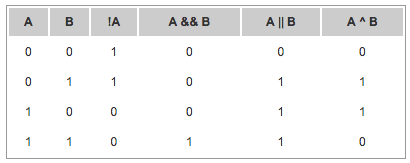
\includegraphics[width=.85\textwidth]{figuras/boolean.png}
		\caption{Topcoder}
	\end{figure}
\end{center}

\end{block}

\end{frame}

%- - - - - - - - - - - - - - - - - - - - - - - - - - - - - - - - - SLIDE -
\begin{frame}
\frametitle{Estruturas de Dados (continuação)}
\begin{block}{Bitmask}
A versão bit a bit destas operações funciona da mesma forma, mas ao invés de interpretar seus argumentos como verdadeiro ou falso, eles operam sobre cada bit dos argumentos. Logo, se A é 1010 e B é 1100, então:
\begin{itemize}
	\bitem A \& B = 1000
	\bitem A | B = 1110
	\bitem A \^\ B = 0110
	\bitem $\sim$A = 11110101 (o numero de 1's depende no número de bits do tipo de A).
\end{itemize}
\end{block}
\end{frame}

%- - - - - - - - - - - - - - - - - - - - - - - - - - - - - - - - - SLIDE -
\begin{frame}
\frametitle{Estruturas de Dados (continuação)}
\begin{block}{Bitmask}
\begin{itemize}
	\bitem Outros dois operadores que precisaremos são os \textit{shift operators} $a << b$ e $a >> b$. O primeiro faz um \textit{shift} de todos os bits em $a$ para a esquerda por $b$ posições. O segundo faz a mesma coisa mas o \textit{shift} é pra direita.
	\bitem Para valores não negativos (que são os que estamos interessados), os novos bits que aparecem com os \textit{shifts} são zeros.
	\bitem Podemos considerar \textit{shifts} de $b$ bits para a esquerda como uma multiplicação por $2^b$ e para a direira como divisão inteira por $2^b$.
	\bitem Um dos usos mais comuns de \textit{shifts} bit a bit são para acessar um bit em particular. Por exemplo, $1 << x$ é um número binário com o bit $x$ setado e os outros não setados(bits são quase sempre contados como sendo o menos significante o mais a direita, o qual tem índice 0).
\end{itemize}
\end{block}
\end{frame}

%- - - - - - - - - - - - - - - - - - - - - - - - - - - - - - - - - SLIDE -
\begin{frame}
\frametitle{Estruturas de Dados (continuação)}
\begin{block}{Bitmask}
\begin{itemize}
	\bitem Em geral, usamos um inteiro para representar um conjunto em um domínio de até 32 valores (ou 64, usando um inteiro de 64 bits), com um bit setado representando um valor que está presente no conjunto e um bit não setado representando um valor que não está presente no conjunto.
	\bitem Sabendo disso, as seguintes operações são bem intuitivas, onde ALL\_BITS é um número com 1's para todos os bits correspondendo aos elementos do domínio:
	\begin{itemize}
		\bitem União de conjuntos: A | B
		\bitem Intersecção de conjuntos: A \& B
		\bitem Subtração de conjuntos: A \& $\sim$B
		\bitem Negação de conjuntos: ALL\_BITS \^\ A
		\bitem Setar um bit: A |= 1 << bit
		\bitem Limpar um bit: A \&= $\sim$(1 << bit)
		\bitem Testar um bit: (A \& 1 << bit) != 0
	\end{itemize}
\end{itemize}
\end{block}
\end{frame}

%- - - - - - - - - - - - - - - - - - - - - - - - - - - - - - - - - SLIDE -
\begin{frame}
\frametitle{Estruturas de Dados (continuação)}
\begin{block}{Bitset}
\begin{itemize}
	\bitem Esta representação com inteiros entretanto é muito limitada, sendo esta limitação de apenas o maior inteiro representado pela linguagem, que normalmente é um inteiro de 64 bits.
	\bitem Para lidar com conjuntos maiores, existe uma implementação na STL que satisfaz esta necessidade com alguma perda de performance chamada \textit{bitset}.
\end{itemize}
\end{block}

\end{frame}

%- - - - - - - - - - - - - - - - - - - - - - - - - - - - - - - - - SLIDE -
\begin{frame}
\frametitle{Estruturas de Dados (continuação)}
\begin{block}{Bitset}
\begin{itemize}
	\bitem Operadores usados nas bitmasks também podem ser usados com bitsets:
	\begin{itemize}
		\bitem \&, |, \^\ , <<, >>, $\sim$
	\end{itemize}
	\bitem Além destes, vários outras funcionalidades são implementadas
\end{itemize}
\end{block}
\end{frame}

%- - - - - - - - - - - - - - - - - - - - - - - - - - - - - - - - - SLIDE -
\begin{frame}
\frametitle{Estruturas de Dados (continuação)}
\begin{block}{Bitset}
\begin{itemize}
	\bitem Acesso a bits pelo operador [ ]
	\bitem set() -- Seta os bits do bitset
	\bitem reset() -- Reseta os bits do bitset
	\bitem flip() -- Inverte os bits do bitset
	\bitem to\_ulong() -- Retorna o bitset convertido para um unsigned long
	\bitem to\_string() -- Retorna o bitset convertido para uma string
	\bitem count() -- Retorna o número de bits ativos
	\bitem size() -- Retorna o número de bits do bitset
	\bitem test(pos) -- Retorna se o bit na posição \textit{pos} está setado
\end{itemize}
\end{block}
\end{frame}
%- - - - - - - - - - - - - - - - - - - - - - - - - - - - - - - - - SLIDE -
\begin{frame}
\frametitle{Leituras Recomendadas}

\begin{block}{}
\begin{itemize}
\tiny
	\bitem \url{http://community.topcoder.com/tc?module=Static&d1=tutorials&d2=bitManipulation}
	\bitem \url{http://www.codechef.com/wiki/tutorial-bitwise-operations}
	\bitem \url{http://www.comp.nus.edu.sg/~stevenha/visualization/bitmask.html}
	\bitem \url{http://inf.ufg.br/~paulocosta/tap/material/bitmask.pdf}
\end{itemize}
\end{block}

\end{frame}



% ----------------------------------------------------------------------- AULA 4 ----------
\section{Aula 4\ \ \ \ \ \ \ \ \ \ \ \ \ \ \ \ \ \ \ \ \ \ \ \ \ \ \ \ \ \ \ \ \ \ \ \ \ \ \ \ \ \ \ \ \  Complete Search}
%- - - - - - - - - - - - - - - - - - - - - - - - - - - - - - - - - SLIDE -
\begin{frame}
\frametitle{Complete Search}
\begin{block}{}
\begin{itemize}
	\bitem Estratégia baseada no princípio KISS (``Keep It Simple, Stupid'')
	\begin{itemize}
		\bitem Buscar os resultados evitando qualquer complexidade desnecessária.
	\end{itemize}
	\bitem O objetivo numa competição de programação é escrever um programa que resolva o problema dentro do tempo limite.
	\begin{itemize}
		\bitem Não importa se existe ou não uma solução mais eficiente.
	\end{itemize}
	\bitem A busca exaustiva faz uso do método trivial, de força bruta, todas as possíveis soluções são analisadas para encontrar a resposta.
	\bitem Essa técnica sempre deve ser a primeira a ser considerada.
	\begin{itemize}
		\bitem Caso funcione dentro do limite de tempo / memória, use-a! 
		\begin{itemize}
			\bitem Geralmente é fácil de codificar e debugar.
%			\bitem Mais tempo para trabalhar nos problemas difíceis. 
		\end{itemize}
	\end{itemize}
	\bitem Apenas alguns milhões de possíveis respostas para um problema? Itere em todas elas e encontre aquela que funciona.
\end{itemize}
\end{block}
\pause

\begin{block}{\tiny Cuidado!!}
Nem sempre é óbvio que a busca exaustiva pode ser usada.
\end{block}
\end{frame}

%- - - - - - - - - - - - - - - - - - - - - - - - - - - - - - - - - SLIDE -
\begin{frame}
\frametitle{Complete Search}

\begin{block}{}
\begin{itemize}
	\bitem Uma das técnicas de resolução de problemas mais importantes;
	\begin{itemize}
		\bitem Pode ser aplicada a uma grande gama de problemas quando as instâncias são pequenas os suficiente
		\bitem Ponto de partida para o desenvolvimento de outros algoritmos.
	\end{itemize}
	\bitem Competidor precisa saber:
	\begin{itemize}
		\bitem Gerar/testar: subconjuntos, permutações, ...
		\bitem Técnicas para reduzir o espaço de busca
		\bitem Estimar a complexidade no pior caso
	\end{itemize}
	\bitem Ajustes no código podem influenciar bastante no tempo de execução;
	\begin{itemize}
		\bitem Vale a pena implementar a mesma solução de formas diferentes.
	\end{itemize}
\end{itemize}	
\end{block}

\begin{block}{\tiny \#protip}
Quando não conseguir pensar em um jeito melhor de resolver o problema arrisque a solução por força bruta.
Caso exista um caso onde ela não é rápida o suficiente, mantenha a solução por perto e use-a para testar outras soluções nos casos menores.
\end{block}
\end{frame}

%- - - - - - - - - - - - - - - - - - - - - - - - - - - - - - - - - SLIDE -
\begin{frame}
\frametitle{Complete Search}
\begin{block}{Filtrar vs. Gerar }
Duas possíveis abordagens podem ser escolhidas quando fazendo uma busca exaustiva:
\begin{itemize}
	\bitem Filtragem -- Todas as possíveis soluções são geradas e depois examinadas para eliminar as inválidas.
	\bitem Geração -- Soluções construídas progressivamente, assim que uma inconsistência é detectada a solução é descartada.
\end{itemize}
\end{block}
\pause
\begin{block}{}
\begin{itemize}
	\bitem Candidato parcial (estado) -- parte de uma possível solução;
	\begin{itemize}
		\bitem Pode ser completado (através de um passo de extensão) de diferentes maneiras para gerar uma solução.
	\end{itemize}	
	\bitem Candidatos são os nós de uma árvore. Cada candidato parcial é pai dos candidatos que podem ser obtidos a partir dele em um passo de extensão.
\end{itemize}
\end{block}
\end{frame}

%- - - - - - - - - - - - - - - - - - - - - - - - - - - - - - - - - SLIDE -
\begin{frame}
\frametitle{Complete Search}
\begin{center}
\begin{figure}
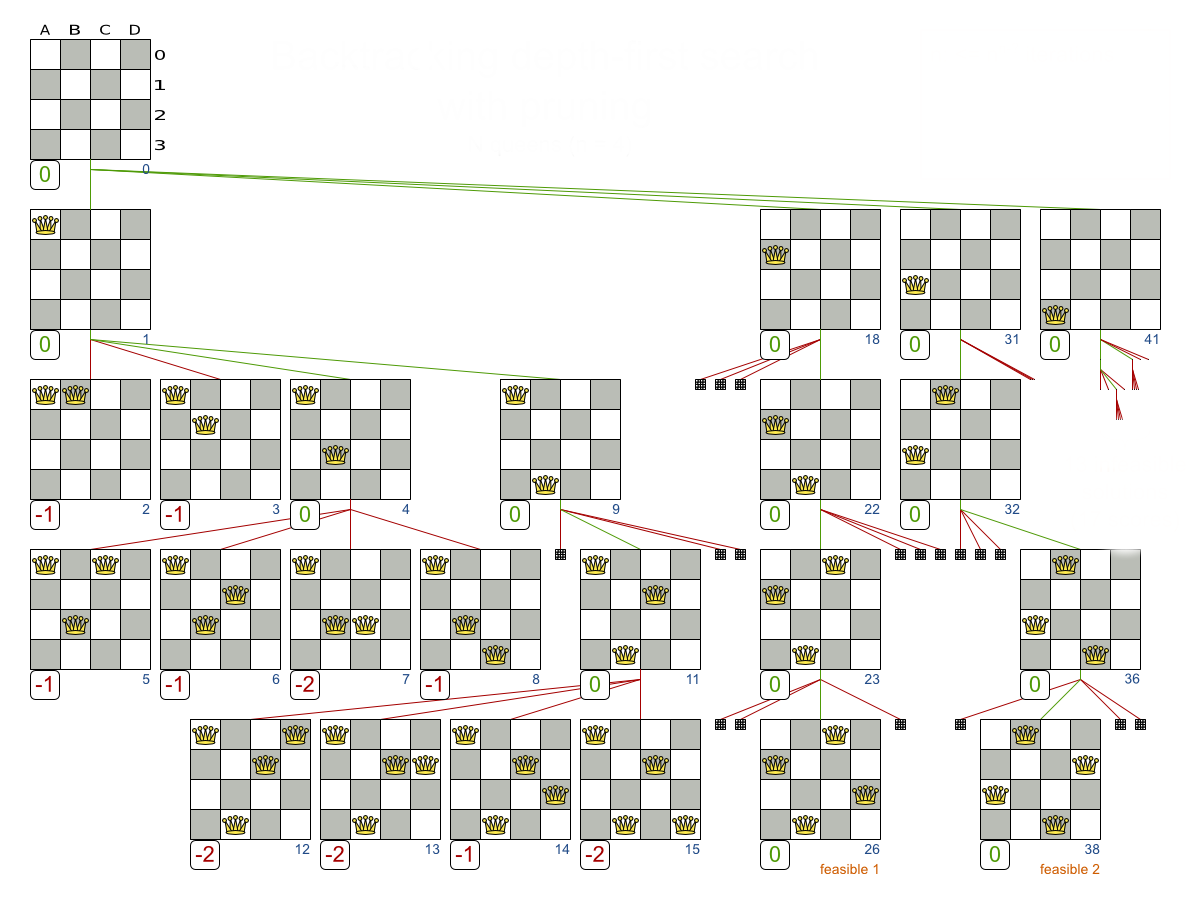
\includegraphics[width=.9\textwidth]{figuras/backtrackingDepthFirstSearchNQueens.png}
\end{figure}
\end{center}
\end{frame}

%- - - - - - - - - - - - - - - - - - - - - - - - - - - - - - - - - SLIDE -
\begin{frame}
\frametitle{Complete Search}
\begin{block}{Problema: $n$ Queens}
\scriptsize
Colocar $n$ rainhas em um tabuleiro de xadrez $n\ x\ n$ de modo que uma rainha não ataque outra.
\end{block}
\pause
\begin{block}{Abordagens..}
\begin{itemize}[<+->]
	\bitem 1. Gerar $n$ pares $(x,y)$ e verificar se formam uma solução válida.
	\begin{itemize}
		\item[] $n^{2n}$ -- \textbf{\textcolor{red}{BAD!}}
	\end{itemize}
	\bitem \texttt{$Obs_1$.: Cada coluna deve ter exatamente uma rainha..}
	\bitem 2. Gerar as $n^n$ possíveis soluções e verificar se são válidas.
	\begin{itemize}
		\item[] \textbf{Melhorou, só que não!}
	\end{itemize}
	\bitem \texttt{$Obs_2$.: Cada linha também tem exatamente uma rainha..}
	\bitem 3. Gerar as $n!$ possíveis soluções e verificar se são válidas.
	\begin{itemize}
		\item[] \textbf{Hmm, parece ``bom''.. será que dá pra melhorar?}
	\end{itemize}
\end{itemize}
\end{block}
\end{frame}

%- - - - - - - - - - - - - - - - - - - - - - - - - - - - - - - - - SLIDE -
\begin{frame}
\frametitle{Complete Search}
\begin{block}{Problema: $n$ Queens}
\scriptsize
Colocar $n$ rainhas em um tabuleiro de xadrez $n\ x\ n$ de modo que uma rainha não ataque outra.
\end{block}

\begin{block}{Busca em profundidade, Backtracking}
\begin{itemize}[<+->]
	\bitem Podemos tentar adicionar as rainhas uma por uma, recursivamente, no tabuleiro.
	\bitem Explorando o fato de que é necessário colocar uma rainha por coluna, em cada passo da recursão basta escolher em qual linha na coluna atual colocar a rainha.
	\bitem Não faz sentido colocar uma rainha em uma posição que entra na zona de ataque de alguma das rainhas anteriormente colocadas.
	\bitem Continuamos tentando gerar as $n!$ permutações, mas agora só geramos aquelas que são válidas. \color{ccomments}{(filtrar vs. gerar)}
\end{itemize}
\end{block}
\end{frame}

%- - - - - - - - - - - - - - - - - - - - - - - - - - - - - - - - - SLIDE -
\begin{frame}
\frametitle{Complete Search}
\begin{block}{Problema: $n$ Queens}
\scriptsize
Colocar $n$ rainhas em um tabuleiro de xadrez $n\ x\ n$ de modo que uma rainha não ataque outra.
\end{block}

\begin{block}{Busca em profundidade, Backtracking}
\includefile{c++}{codes}{pseudonqueen.cpp}
\end{block}
\end{frame}

%- - - - - - - - - - - - - - - - - - - - - - - - - - - - - - - - - SLIDE -
\begin{frame}
\frametitle{Complete Search}

\begin{block}{Busca em profundidade, Backtracking}

\begin{itemize}
	\bitem Essa abordagem é um exemplo de uma busca em profundidade (DFS - \emph{Depth First Search})
	\begin{itemize}
		\bitem O algoritmo tenta iterar do topo ao fundo da árvore o mais rápido possível.
		\bitem Um vez que $k$ rainhas são colocadas no tabuleiro, apenas tabuleiros com mais rainhas são examinados.
	\end{itemize}
	\bitem O algoritmo busca na árvore de cima para baixo, analisando os candidatos parciais.
	\bitem Quando uma solução é encontrada ou uma inconsistência detectada, o mecanismo de \emph{backtracking} entra em ação
	\begin{itemize}
		\bitem O caminho que levou até aquela solução é percorrido ao contrário até que uma nova extensão possa ser gerada.
	\end{itemize}
\end{itemize}
\end{block}
\end{frame}

%- - - - - - - - - - - - - - - - - - - - - - - - - - - - - - - - - SLIDE -
\begin{frame}
\frametitle{Complete Search}
	\begin{center}
		\begin{figure}
			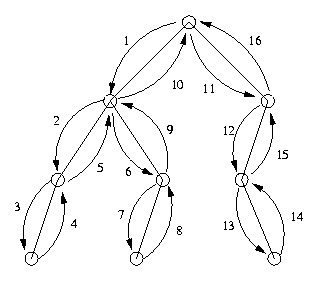
\includegraphics[width=.52\textwidth]{figuras/dfs.png}
			\caption{USACO}
		\end{figure}
	\end{center}
\end{frame}

%- - - - - - - - - - - - - - - - - - - - - - - - - - - - - - - - - SLIDE -
\begin{frame}
\frametitle{Complete Search}

\begin{block}{Busca em profundidade, Backtracking - Complexidade}

\begin{itemize}
	\bitem Seja $d$ o número de decisões que devem ser feitas 
	\begin{itemize}
		\item[] \scriptsize{No caso das $n$-rainhas $d=n$, o nro. de colunas que devemos preencher.}
	\end{itemize}
	\bitem Seja $C$ a quantidade de escolhas para cada decisão
	\begin{itemize}
		\item[] \scriptsize{No caso das $n$-rainhas $C=n$, já que qualquer uma das linhas pode ser escolhida.}
	\end{itemize}
	\bitem No pior caso, a busca leva tempo $O(C^d)$, ou seja, uma quantidade exponencial de tempo.
	\bitem Entretanto, a quantidade de espaço necessária é bem pequena.
	\begin{itemize}
		\bitem Como só é necessário manter informação das decisões a serem feitas, apenas $O(d)$ espaço é necessário.
	\end{itemize}
\end{itemize}
\end{block}
\end{frame}

%- - - - - - - - - - - - - - - - - - - - - - - - - - - - - - - - - SLIDE -
\begin{frame}
\frametitle{Complete Search}
\begin{block}{Problema: Knight Cover}
\scriptsize
Colocar o menor número de cavalos em um tabuleiro de xadrez $n\ x \ n$ de modo que toda célula do tabuleiro está sob ataque.
\tiny{\emph{*Um cavalo não ataca a posição onde ele se encontra.}}
\end{block}
\pause
\begin{block}{Busca em Largura}
\begin{itemize}[<+->]
	\bitem Como queremos o menor número de cavalos, é mais interessante examinar todas as soluções com $k$ cavalos
	antes de partir para aquelas com $k+1$.
	\bitem Essa abordagem é um exemplo de uma busca em largura (BFS - \emph{Breadth First Search})
	\bitem Geralmente a implementação envolve uma fila de estados / candidatos parciais
\end{itemize}
\end{block}
\end{frame}

%- - - - - - - - - - - - - - - - - - - - - - - - - - - - - - - - - SLIDE -
\begin{frame}
\frametitle{Complete Search}
	\begin{center}
		\begin{figure}
			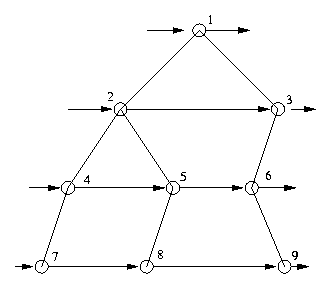
\includegraphics[width=.52\textwidth]{figuras/bfs.png}
			\caption{USACO}
		\end{figure}
	\end{center}
\end{frame}

%- - - - - - - - - - - - - - - - - - - - - - - - - - - - - - - - - SLIDE -
\begin{frame}
\frametitle{Complete Search}
\begin{block}{Busca em Largura}
\includefile{c++}{codes}{pseudobfs.cpp}
\end{block}
\end{frame}

%- - - - - - - - - - - - - - - - - - - - - - - - - - - - - - - - - SLIDE -
\begin{frame}
\frametitle{Complete Search}
\begin{block}{Busca em largura}
\begin{itemize}
	\bitem Chamada de busca em largura porque percorre uma linha inteira (a largura) da árvore de candidatos antes de passar para a próxima linha.
	\bitem Primeiro visita a raiz, então todos os nós no nível 1, depois todos no nível 2, ...
\end{itemize}
\end{block}
\pause
\begin{block}{Busca em largura -- Complexidade}
\begin{itemize}
	\bitem Complexidade de tempo é a mesma da busca em profundidade.
	\bitem Consumo de espaço proporcional ao número de candidatos.
	\begin{itemize}
		\bitem Sejam $c$ o número de escolhas para cada decisão, e $k$ o número de decisões que devem ser feitas.
		\bitem Existem $c^k$ possíveis candidatos que vão estar na fila para o próximo passo.
	\end{itemize}
\end{itemize}
\end{block}
\end{frame}

%- - - - - - - - - - - - - - - - - - - - - - - - - - - - - - - - - SLIDE -
\begin{frame}
\frametitle{Complete Search}
\begin{block}{Busca em aprofundamento iterativo}
\begin{itemize}	\bitem \emph{Depth First with Iterative Deepening} (ID)
	\bitem Alternativa a busca em largura
	\bitem São executadas sequencialmente $D$ buscas em profundidade
	\bitem Cada busca pode ir um nível além da busca anterior
	\bitem Simula uma busca em largura, complexidade de tempo pior mas gasta menos espaço
\end{itemize}
\end{block}
\end{frame}

%- - - - - - - - - - - - - - - - - - - - - - - - - - - - - - - - - SLIDE -
\begin{frame}
\frametitle{Complete Search}
\begin{block}{Busca em aprofundamento iterativo}
\includefile{c++}{codes}{pseudoid.cpp}
\end{block}
\end{frame}

%- - - - - - - - - - - - - - - - - - - - - - - - - - - - - - - - - SLIDE -
\begin{frame}
\frametitle{Complete Search}
\begin{block}{Busca em aprofundamento iterativo -- Complexidade}

\begin{itemize}
	\bitem Complexidade de espaço é a mesma da busca em profundidade;
	\bitem Complexidade de tempo pior:
	\begin{itemize}
		\bitem Busca em profundidade parando na profundidade $k$ leva $O(c^k)$
		\bitem Seja $d$ o número máximo de decisões (profundidade máxima), o tempo gasto será $c^0 + c^1 + c^2 + c^3 + ... + c^d$
	\end{itemize}
	\bitem Sempre que há pelo menos duas escolhas a serem tomadas, a busca em aprofundamento iterativo
	não gasta mais que o dobro de tempo que a busca em largura teria gasto.
\end{itemize}	

\end{block}
\end{frame}

%- - - - - - - - - - - - - - - - - - - - - - - - - - - - - - - - - SLIDE -
\begin{frame}
\frametitle{Complete Search}
\begin{block}{Quando usar?}
\begin{table}
    \begin{tabular}{|p{2.5cm}|l|l|p{5cm}|}
        \hline
        Busca                    & Tempo    & Espaço    & Quando usar                                                                                                                \\ \hline
        Profundidade             & $O(c^k)$ & $O(k)$    & a) De qualquer maneira vai olhar todos os estados, b) sabe o nível que a resposta está, ou c) não está procurando a menor resposta. \\ \hline
        Largura                  & $O(c^d)$ & $O(c^d)$  & a) Sabe que a resposta fica perto do topo da árvore, ou b) está procurando a menor resposta.                                     \\ \hline
        Aprofundamento Iterativo & $O(c^d)$ & $O(d)$    & Quer fazer uma busca em largura, não tem espaço e pode gastar um pouco mais de tempo.                                       \\
        \hline
    \end{tabular}
\end{table}
\end{block}
\end{frame}

\subsection{Hora de resolver alguns problemas..}

%- - - - - - - - - - - - - - - - - - - - - - - - - - - - - - - - - SLIDE -
\begin{frame}
\frametitle{Complete Search}
\begin{block}{The Clocks [IOI 94]}
\begin{itemize}
	\bitem Existem 9 relógios em um \emph{grid} $3\ x\ 3$; que podem estar mostrando um dos seguintes horários: 12:00, 3:00, 6:00 ou 9:00.
	\bitem Objetivo: Fazer com que todos mostrem 12:00.
	\bitem 9 comandos podem ser usados para manipular os relógios
	\begin{itemize}
		\bitem Cada comando rotaciona um subconjunto de relógios 90 graus no sentido horário. 
	\end{itemize}
	\bitem Qual a menor sequência de comandos que faz com que todos os relógios mostrem 12:00.
\end{itemize}
\end{block}
\pause
\begin{block}{}
\begin{itemize}
	\bitem Solução mais óbvia: fazer movimentos 
	\bitem 
\end{itemize}
\end{block}

%A group of nine clocks inhabits a 3 x 3 grid; each is set to 12:00, 3:00, 6:00, or 9:00. Your goal is to manipulate them all to read 12:00. Unfortunately, the only way you can manipulate the clocks is by one of nine different types of move, each one of which rotates a certain subset of the clocks 90 degrees clockwise.
%
%Find the shortest sequence of moves which returns all the clocks to 12:00.
%
%The ``obvious'' thing to do is a recursive solution, which checks to see if there is a solution of 1 move, 2 moves, etc. until it finds a solution. This would take 9k time, where k is the number of moves. Since k might be fairly large, this is not going to run with reasonable time constraints.
%
%Note that the order of the moves does not matter. This reduces the time down to k9 , which isn't enough of an improvement.
%
%However, since doing each move 4 times is the same as doing it no times, you know that no move will be done more than 3 times. Thus, there are only 49 possibilities, which is only 262,072, which, given the rule of thumb for run-time of more than 10,000,000 operations in a second, should work in time. The brute-force solution, given this insight, is perfectly adequate.
\end{frame}

%- - - - - - - - - - - - - - - - - - - - - - - - - - - - - - - - - SLIDE -
\begin{frame}
\frametitle{Complete Search}
\begin{block}{UVa 725 -- Division}
%	Encontrar dois numeros de 5 dígitos tais que, abcde / fghij = N
%	cada digito de 0-9 deve aparecer exatamente uma vez, 2  <= N <= 79
%Solução: 
%	testar todos os fghij
%	abcde = fghij*N
%	verifica restrição de uso dos digitos
\end{block}
\end{frame}

%- - - - - - - - - - - - - - - - - - - - - - - - - - - - - - - - - SLIDE -
\begin{frame}
\frametitle{Complete Search}
\begin{block}{Superprime Rib [USACO 1994 Final Round, adapted]}
%
%A number is called superprime if it is prime and every number obtained by chopping some number of digits from the right side of the decimal expansion is prime. For example, 233 is a superprime, because 233, 23, and 2 are all prime. Print a list of all the superprime numbers of length n, for n <= 9. The number 1 is not a prime.
%
%For this problem, use depth first search, since all the answers are going to be at the nth level (the bottom level) of the search.
\end{block}
\end{frame}

%- - - - - - - - - - - - - - - - - - - - - - - - - - - - - - - - - SLIDE -
\begin{frame}
\frametitle{Complete Search}
\begin{block}{Betsy's Tour [USACO 1995 Qualifying Round]}
%A square township has been partitioned into n 2 square plots. The Farm is located in the upper left plot and the Market is located in the lower left plot. Betsy takes a tour of the township going from Farm to Market by walking through every plot exactly once. Write a program that will count how many unique tours Betsy can take in going from Farm to Market for any value of n <= 6.
%
%Since the number of solutions is required, the entire tree must be searched, even if one solution is found quickly. So it doesn't matter from a time perspective whether DFS or BFS is used. Since DFS takes less space, it is the search of choice for this problem.
\end{block}
\end{frame}

%- - - - - - - - - - - - - - - - - - - - - - - - - - - - - - - - - SLIDE -
\begin{frame}
\frametitle{Complete Search}
\begin{block}{UVa 11742 -- Social Constraints}
%	0 < n <= 8 amigos vão ao cinema
%	vão se sentar na primeira fileira, com n assentos consecutivos
%	Existem 0 <= m <= 20 restrições, (a,b,c) indicando que a e b devem estar sentados no máximo a c assentos de distancia
%	De quantas formas eles podem se sentar?
%Solução
%	testar as n! permutações
%	verifica se a permutação satisfaz todas as restrições
\end{block}
\end{frame}

%- - - - - - - - - - - - - - - - - - - - - - - - - - - - - - - - - SLIDE -
\begin{frame}
\frametitle{Complete Search}
\begin{block}{UVa 12346 - Water Gate Management}
%	uma barragem tem 1 <= n <= 20 portões que deixam a água passar quando necessário, cada portão tem uma taxa que determina quanta água ele é capaz de deixar passar por segundo e um custo de abertura.
%	Sua tarefa é controlar a abertura dos portões de modo que a agua possa fluir a uma taxa de x unidades por segundo e o custo total de abertura seja minimo.
%Solução
%	testar todos os 2^n subconjuntos de portões que podem ser abertos
%	para cada subconjunto
%		verifica se a taxa passando é maior ou igual a taxa desejada
%			em caso positivo, verifique se o custo é menor que o menor custo encontrado ate agora
\end{block}
\end{frame}

%- - - - - - - - - - - - - - - - - - - - - - - - - - - - - - - - - SLIDE -
\begin{frame}
\frametitle{Complete Search}
\begin{block}{Party Lamps [IOI 98]}
%You are given N lamps and four switches. The first switch toggles all lamps, the second the even lamps, the third the odd lamps, and last switch toggles lamps 1, 4, 7, 10, ... .
%
%Given the number of lamps, N, the number of button presses made (up to 10,000), and the state of some of the lamps (e.g., lamp 7 is off), output all the possible states the lamps could be in.
%
%Naively, for each button press, you have to try 4 possibilities, for a total of 410000 (about 106020 ), which means there's no way you could do complete search (this particular algorithm would exploit recursion).
%
%Noticing that the order of the button presses does not matter gets this number down to about 100004 (about 1016 ), still too big to completely search (but certainly closer by a factor of over 106000 ).
%
%However, pressing a button twice is the same as pressing the button no times, so all you really have to check is pressing each button either 0 or 1 times. That's only 24 = 16 possibilities, surely a number of iterations solvable within the time limit.
\end{block}
\end{frame}

%- - - - - - - - - - - - - - - - - - - - - - - - - - - - - - - - - SLIDE -
\begin{frame}
\frametitle{Complete Search}
\begin{block}{Addition Chains}
%An addition chain is a sequence of integers such that the first number is 1, and every subsequent number is the sum of some two (not necessarily unique) numbers that appear in the list before it. For example, 1 2 3 5 is such a chain, as 2 is 1+1, 3 is 2+1, and 5 is 2+3. Find the minimum length chain that ends with a given number.
%
%Analysis: Depth-first search with iterative deepening works well here, as DFS has a tendency to first try 1 2 3 4 5 ... n, which is really bad and the queue grows too large very quickly for BFS.
\end{block}
\end{frame}

%- - - - - - - - - - - - - - - - - - - - - - - - - - - - - - - - - SLIDE -
\begin{frame}
\frametitle{Complete Search}
\begin{block}{Dicas}
\begin{itemize}[<+->]
	\bitem Podar o quanto antes
	\bitem Aproveitar simetrias
	\bitem Pré-cálculo
%	\bitem Inverter o problema (?)
	\bitem Otimizar código
	\bitem Usar um algoritmo/estrutura de dados melhor
\end{itemize}
\end{block}
\end{frame}

%- - - - - - - - - - - - - - - - - - - - - - - - - - - - - - - - - SLIDE -
\begin{frame}
\frametitle{Leituras Recomendadas}

\begin{block}{}
\begin{itemize}
\scriptsize
	\bitem \url{http://community.topcoder.com/tc?module=Static&d1=tutorials&d2=recursionPt1}
	\bitem \url{http://community.topcoder.com/tc?module=Static&d1=tutorials&d2=recursionPt2}
	\bitem \url{http://www.inf.ufg.br/~paulocosta/tap/material/bt1.pdf}
	\bitem \url{http://www.inf.ufg.br/~paulocosta/tap/material/bt2.pdf}
%	\bitem \url{http://www.inf.ufg.br/~paulocosta/tap/material/bt3.pdf} % MITM
	\bitem \url{http://www.comp.nus.edu.sg/~stevenha/visualization/recursion.html}
\end{itemize}
\end{block}

\end{frame}


\end{document}

